\documentclass[11pt,a4paper]{article}

\usepackage[utf8]{inputenc}
\usepackage[T1]{fontenc}
\usepackage{lmodern}
\usepackage[margin=2.5cm]{geometry}
\usepackage{amsmath,amssymb}
\usepackage{booktabs,tabularx,array}
\usepackage{xcolor}
\usepackage{tikz}
\usetikzlibrary{positioning,arrows.meta,fit,backgrounds,shapes.geometric,calc}
\usepackage{listings}
\usepackage{enumitem}
\usepackage{caption}
\usepackage{float}
\usepackage{fancyhdr}
\usepackage[hidelinks]{hyperref}

% --- Nombres en español (sin babel) ---------------------------------------
\renewcommand{\contentsname}{Índice}
\renewcommand{\tablename}{Tabla}
\renewcommand{\figurename}{Figura}
\renewcommand{\refname}{Referencias}
\renewcommand{\lstlistingname}{Código}

\definecolor{azul}{HTML}{1F4E79}
\definecolor{verde}{HTML}{2E7D32}
\definecolor{rojo}{HTML}{C62828}
\definecolor{naranja}{HTML}{EF6C00}
\definecolor{gris}{HTML}{F4F6F8}

\lstset{
  language=Python, basicstyle=\ttfamily\footnotesize, keywordstyle=\color{azul}\bfseries,
  commentstyle=\color{gray}\itshape, stringstyle=\color{verde}, backgroundcolor=\color{gris},
  frame=single, rulecolor=\color{gray!40}, breaklines=true, numbers=left,
  numberstyle=\tiny\color{gray}, showstringspaces=false, inputencoding=utf8, extendedchars=true,
  literate={á}{{\'a}}1 {é}{{\'e}}1 {í}{{\'i}}1 {ó}{{\'o}}1 {ú}{{\'u}}1 {ñ}{{\~n}}1
           {Á}{{\'A}}1 {É}{{\'E}}1 {Í}{{\'I}}1 {Ó}{{\'O}}1 {Ú}{{\'U}}1
}

\pagestyle{fancy}
\fancyhf{}
\lhead{\small Agente DevOps de revisión de Pull Requests}
\rhead{\small Tecnology Trend}
\cfoot{\thepage}

\newcommand{\Pdef}{P_{\text{def}}}

\begin{document}
\sloppy

% ============================== PORTADA ===================================
\begin{titlepage}
\centering
{\large FUNDACIÓN UNIVERSITARIA LOS LIBERTADORES\par}
{\large Facultad de Ingeniería y Ciencias Básicas\par}
{\large Ingeniería de Sistemas\par}
\vspace{3cm}
{\Huge\bfseries Agente Inteligente de Revisión de Código y Gestión de Pull Requests\par}
\vspace{0.6cm}
{\Large Proyecto 4 --- DevOps\par}
\vspace{0.4cm}
{\large Taller de Ingeniería de Agentes Inteligentes\par}
\vspace{0.3cm}
{\large\itshape Entrega 2: Diseño arquitectónico y función de utilidad\par}
\vspace{3cm}
{\large\textbf{Presentado por:}\\ Simon Hurtado\par}
\vspace{0.8cm}
{\large\textbf{Docente:}\\ Profesor Gonzalo\par}
\vspace{0.8cm}
{\large\textbf{Asignatura:}\\ Tecnology Trend\par}
\vfill
{\large Bogotá D.C., noviembre de 2026\par}
\end{titlepage}

\tableofcontents
\newpage
\setcounter{section}{2}\setcounter{figure}{1}\setcounter{table}{2}\setcounter{equation}{0}
% ============================== 3 =========================================
\section{Diseño arquitectónico}

\subsection{Justificación del enfoque}

Se eligió una \textbf{arquitectura basada en utilidad}. Un agente reflejo simple (reglas
\textit{if/else}) no puede equilibrar objetivos en conflicto: tendría que decidir de forma binaria si
un PR de 1200 líneas en el módulo de autenticación ``es aceptable'' o no. Un agente basado en
objetivos solo sabría que la meta es ``PR cerrado'', sin distinguir entre cerrarlo rápido y cerrarlo
bien. La función de utilidad, en cambio, asigna a cada acción un valor numérico que combina
velocidad, riesgo, costo humano y calidad, y permite \emph{auditar} cada decisión.

Además, por ser el entorno parcialmente observable, el agente mantiene un \textbf{modelo del mundo}
que convierte los sensores en una estimación de $\Pdef(s)$. Sobre esta base se añade una \textbf{capa
de restricciones duras} (penalización $w_p$) que impide, sin importar el resto de términos, fusionar
código con pruebas rotas o con vulnerabilidades críticas. La arquitectura queda preparada para
evolucionar a un esquema híbrido: el modelo de riesgo $\Pdef$ es el componente que podría sustituirse
por un modelo de aprendizaje automático entrenado con el historial de incidentes, sin modificar la
capa de utilidad.

\subsection{Flujo interno de decisión}

\begin{figure}[H]
\centering
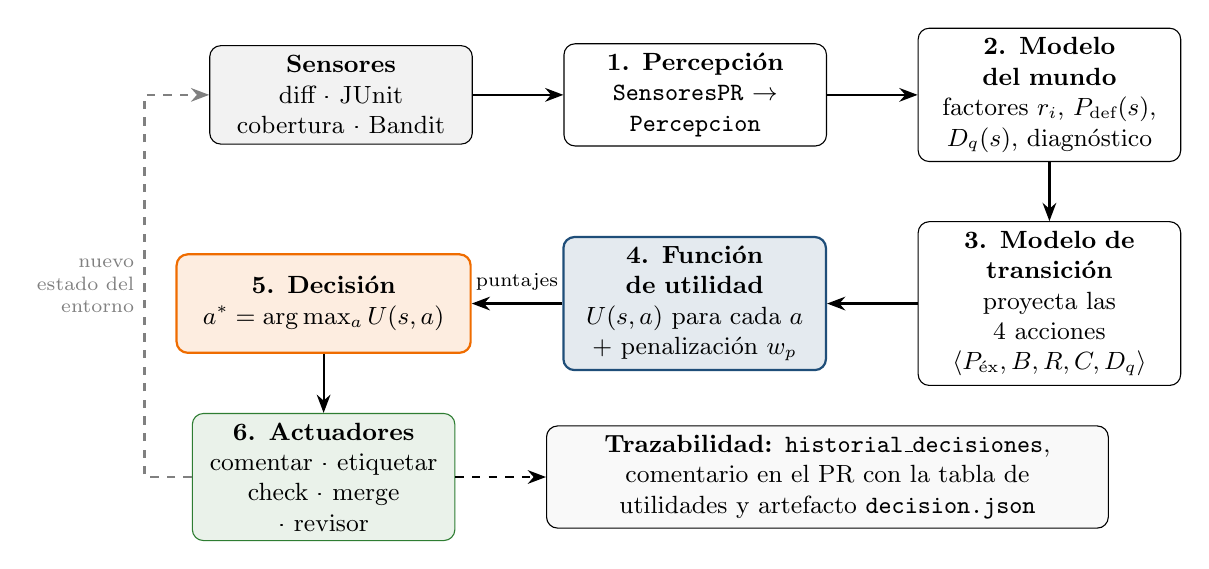
\begin{tikzpicture}[
  node distance=0.75cm and 1.15cm, >=Stealth,
  m/.style={draw, rounded corners, align=center, text width=3.1cm, minimum height=1.25cm, font=\small, fill=white},
  s/.style={m, fill=gray!10},
  u/.style={m, fill=azul!12, draw=azul, thick},
  d/.style={m, fill=naranja!12, draw=naranja, thick},
  a/.style={m, fill=verde!10, draw=verde},
  flecha/.style={->, thick}]
% Sensores
\node[s] (s1) {\textbf{Sensores}\\diff · JUnit\\cobertura · Bandit};
\node[m, right=of s1] (p) {\textbf{1. Percepción}\\\texttt{SensoresPR} $\to$\\\texttt{Percepcion}};
\node[m, right=of p] (mw) {\textbf{2. Modelo del mundo}\\factores $r_i$, $\Pdef(s)$,\\$D_q(s)$, diagnóstico};
\node[m, below=of mw] (tr) {\textbf{3. Modelo de transición}\\proyecta las 4 acciones\\$\langle P_{\text{éx}}, B, R, C, D_q\rangle$};
\node[u, left=of tr] (U) {\textbf{4. Función de utilidad}\\$U(s,a)$ para cada $a$\\+ penalización $w_p$};
\node[d, left=of U, text width=3.5cm] (dec) {\textbf{5. Decisión}\\\mbox{$a^* = \arg\max_a U(s,a)$}};
\node[a, below=of dec] (act) {\textbf{6. Actuadores}\\comentar · etiquetar\\check · merge · revisor};
\node[m, right=of act, text width=6.9cm, fill=gray!5] (log) {\textbf{Trazabilidad:} \texttt{historial\_decisiones}, comentario en el PR con la tabla de utilidades y artefacto \texttt{decision.json}};

\draw[flecha] (s1) -- (p);
\draw[flecha] (p) -- (mw);
\draw[flecha] (mw) -- (tr);
\draw[flecha] (tr) -- (U);
\draw[flecha] (U) -- node[above=1pt, font=\scriptsize]{puntajes} (dec);
\draw[flecha] (dec) -- (act);
\draw[flecha, dashed] (act) -- (log);
\draw[flecha, dashed, gray] (act.west) -- ++(-0.6,0) |- node[pos=0.25, left, font=\scriptsize, align=right]{nuevo\\estado del\\entorno} (s1.west);
\end{tikzpicture}
\caption{Flujo interno del Agente DevOps basado en utilidad.}
\label{fig:arquitectura}
\end{figure}

Los módulos de la figura~\ref{fig:arquitectura} corresponden uno a uno con los métodos de la clase
\texttt{AgenteBasadoEnUtilidad} de la plantilla del taller:

\begin{enumerate}[leftmargin=*]
\item \textbf{Percepción:} \texttt{SensoresPR.a\_percepcion()} normaliza las lecturas del pipeline.
\item \textbf{Modelo del mundo:} \texttt{actualizar\_estado\_interno()} calcula $\Pdef$ y clasifica el PR
      (\texttt{PR\_TRIVIAL}, \texttt{PR\_ESTANDAR}, \texttt{PR\_RIESGOSO}, \texttt{PR\_FALLIDO},
      \texttt{PR\_BLOQUEANTE}).
\item \textbf{Modelo de transición:} \texttt{generar\_estados\_proyectados()} estima el resultado de las
      cuatro acciones. Siempre se generan las cuatro, sin importar el diagnóstico.
\item \textbf{Utilidad:} \texttt{calcular\_utilidad()} aplica la ecuación~\eqref{eq:U}.
\item \textbf{Decisión:} \texttt{seleccionar\_mejor\_accion()} toma el \textit{argmax}.
\item \textbf{Actuadores:} \texttt{ejecutar\_actuador()} y el workflow de GitHub Actions aplican la acción.
\end{enumerate}

% ============================== 4 =========================================
\section{Función de utilidad}

\subsection{Definición formal}

Sea $s$ el estado percibido de un PR y $a \in \mathcal{A} = \{\textsc{merge}, \textsc{corregir},
\textsc{arquitecto}, \textsc{bloquear}\}$. La utilidad de ejecutar $a$ en $s$ es:

\begin{equation}
\label{eq:U}
U(s,a) = w_e\,P_{\text{éx}}(s,a) + w_b\,B(a) - w_r\,R(s,a) - w_c\,C(a) - w_q\,D_q(s,a) - w_p\,\mathbf{1}\big[\text{viola}(s,a)\big]
\end{equation}

\noindent y el agente elige $a^* = \arg\max_{a \in \mathcal{A}} U(s,a)$. Los términos son:

\begin{itemize}[leftmargin=*]
\item $P_{\text{éx}}(s,a) \in [0,1]$: probabilidad de que la acción deje el PR correctamente resuelto.
\item $B(a) \in [0,100]$: beneficio en velocidad de entrega (100 = merge inmediato, 0 = pipeline detenido).
\item $R(s,a) \in [0,1]$: riesgo esperado en producción.
\item $C(a) \in [0,1]$: costo de intervención (tiempo humano de revisión o bloqueo del pipeline).
\item $D_q(s,a) \in [0,1]$: déficit de calidad si el código se fusiona sin cambios (solo aplica a \textsc{merge}).
\item $\mathbf{1}[\text{viola}]$: vale 1 si la acción incumple una política dura de CI/CD.
\end{itemize}

\subsection{Modelo de riesgo $\Pdef(s)$}

Como el entorno es parcialmente observable, la probabilidad de que el PR contenga un defecto se
estima a partir de cinco factores normalizados $r_i(s) \in [0,1]$:

\begin{align}
r_{\text{tests}} &= 1 - \frac{\text{pruebas que pasan}}{\text{pruebas totales}} &
r_{\text{cob}} &= \max\!\Big(0, \frac{0.80 - \text{cob}}{0.80}\Big) \nonumber\\
r_{\text{tam}} &= \min\!\Big(1, \frac{\text{líneas}}{1000}\Big) &
r_{\text{crit}} &= \mathbf{1}[\text{toca módulo crítico}] \nonumber\\
r_{\text{seg}} &= \min\big(1,\; 1.0\,n_{\text{crít}} + 0.5\,n_{\text{alta}} + 0.15\,n_{\text{media}}\big) \nonumber
\end{align}

\begin{equation}
\label{eq:pdef}
\Pdef(s) = \min\Big(1,\; 0.05 + 0.45\,r_{\text{tests}} + 0.15\,r_{\text{cob}} + 0.15\,r_{\text{tam}}
+ 0.10\,r_{\text{crit}} + 0.40\,r_{\text{seg}}\Big)
\end{equation}

\noindent Los módulos críticos se detectan por la ruta del archivo (\texttt{auth}, \texttt{payment},
\texttt{infra}, \texttt{migrations}, \texttt{.github/workflows}, etc.). Si el PR solo modifica
documentación, $r_{\text{tam}} = r_{\text{crit}} = 0$.

El riesgo en producción combina $\Pdef$ con el impacto $I(a)$ de la acción y una exposición
$E(s)$:

\begin{equation}
R(s,a) = \min\big(1,\; \Pdef(s)\cdot I(s,a) + E(s)\big), \qquad
E(s) = \begin{cases} 0.5 & \text{si } n_{\text{crít}} > 0 \text{ y } a \neq \textsc{bloquear}\\ 0 & \text{en otro caso}\end{cases}
\end{equation}

La exposición $E(s)$ modela que un secreto expuesto o una inyección SQL ya constituyen un incidente:
cualquier acción que no detenga el pipeline deja abierta la ventana de explotación.

El déficit de calidad mide el incumplimiento de los estándares del equipo:
\begin{equation}
D_q(s, \textsc{merge}) = \min\Big(1,\; \frac{\max(0,\, 0.70 - \text{cob})}{0.70} + 0.5\,n_{\text{alta}} + 0.1\,n_{\text{media}}\Big)
\end{equation}

\subsection{Proyección de cada acción}

\begin{table}[H]
\centering
\caption{Estados proyectados por el modelo de transición.}
\label{tab:proyeccion}
\small
\begin{tabularx}{\textwidth}{@{}l c c c c X@{}}
\toprule
\textbf{Acción} & $P_{\text{éx}}$ & $B$ & $I$ (impacto) & $C$ & \textbf{Viola política si\ldots} \\
\midrule
\textsc{merge} & $1-\Pdef$ & 100 & 1.0 crítico / 0.6 & 0.0 & pruebas fallan o $n_{\text{crít}}>0$ \\
\textsc{corregir} & 0.90 con hallazgos / 0.50 & 40 & 0.10 & 0.3 & --- \\
\textsc{arquitecto} & 0.97 & 25 & 0.05 & 0.8 & --- \\
\textsc{bloquear} & 0.99 si $n_{\text{crít}}>0$ / 0.30 & 0 & 0 & 0.6 & --- \\
\bottomrule
\end{tabularx}
\end{table}

\textsc{corregir} tiene alta probabilidad de éxito solo cuando existen \emph{hallazgos concretos}
(pruebas que fallan, baja cobertura, alertas): el autor puede arreglarlos con el comentario del bot.
Si el riesgo proviene del tamaño o de la criticidad del módulo, un comentario automático no lo
resuelve y la revisión humana resulta más útil.

\subsection{Pesos y penalizaciones}

\begin{table}[H]
\centering
\caption{Calibración de pesos.}
\label{tab:pesos}
\begin{tabularx}{\textwidth}{@{}c c l X@{}}
\toprule
\textbf{Peso} & \textbf{Valor} & \textbf{Prioridad} & \textbf{Justificación} \\
\midrule
$w_p$ & 1000 & Crítico (restricción) & Nunca fusionar con pruebas rotas o vulnerabilidad crítica. \\
$w_r$ & 400 & Crítico & Un defecto en producción cuesta mucho más que un retraso. \\
$w_q$ & 300 & Alto & Hacer cumplir los estándares de calidad (Performance). \\
$w_e$ & 100 & Alto & Priorizar acciones que realmente resuelven el PR. \\
$w_c$ & 30 & Medio & Penalizar el tiempo de los revisores senior. \\
$w_b$ & 1 & Base & Escala 0--100: recompensa la entrega rápida. \\
\bottomrule
\end{tabularx}
\end{table}

\subsection{Ejemplos de cálculo}

\paragraph{PR-104 (secreto expuesto, 80 líneas).} $r_{\text{seg}}=1$, $r_{\text{tam}}=0.08$, de
modo que $\Pdef = 0.05 + 0.15(0.08) + 0.40(1) = 0.462$.
\begin{align*}
U(\textsc{merge}) &= 100(0.538) + 100 - 400\,(0.462\cdot0.6 + 0.5) - 0 - 0 - 1000 = -1157.08\\
U(\textsc{corregir}) &= 100(0.90) + 40 - 400\,(0.0462 + 0.5) - 30(0.3) = -97.48\\
U(\textsc{arquitecto}) &= 100(0.97) + 25 - 400\,(0.0231 + 0.5) - 30(0.8) = -111.24\\
U(\textsc{bloquear}) &= 100(0.99) + 0 - 0 - 30(0.6) = \mathbf{81.00}
\end{align*}

\paragraph{PR-105 (migración OAuth2, 1200 líneas en \texttt{src/auth}, pruebas en verde).}
$r_{\text{tam}}=1$ y $r_{\text{crit}}=1$, por lo que $\Pdef = 0.05 + 0.15 + 0.10 = 0.30$ e $I=1.0$.
\begin{align*}
U(\textsc{merge}) &= 100(0.70) + 100 - 400(0.30) = 50.00\\
U(\textsc{corregir}) &= 100(0.50) + 40 - 400(0.03) - 30(0.3) = 69.00\\
U(\textsc{arquitecto}) &= 100(0.97) + 25 - 400(0.015) - 30(0.8) = \mathbf{92.00}\\
U(\textsc{bloquear}) &= 100(0.30) - 30(0.6) = 12.00
\end{align*}
Aunque las pruebas pasan, el tamaño y la criticidad hacen que la revisión senior sea la opción
óptima. Esta es exactamente la situación ambigua que una regla \textit{if/else} no resuelve bien.

\begin{thebibliography}{9}
\bibitem{russell} S. Russell y P. Norvig, \textit{Artificial Intelligence: A Modern Approach}, 4.ª ed. Pearson, 2021.
\bibitem{taller} \textit{Taller de Ingeniería de Agentes Inteligentes: de los fundamentos a los sistemas multiagente}. Material de clase, noviembre de 2026.
\end{thebibliography}

\end{document}
